% В этом шаблоне используется класс spbau-diploma. Его можно найти и, если требуется, 
% поправить в файле spbau-diploma.cls
\documentclass{spbau-diploma}
\begin{document}
% Год, город, название университета и факультета предопределены,
% но можно и поменять.
% Если англоязычная титульная страница не нужна, то ее можно просто удалить.
\filltitle{ru}{
    chair              = {Кафедра математических и информационных технологий},
    title              = {Анализ смесей близкородственных
бактериальных штаммов в метагеномных~сериях},
    % Здесь указывается тип работы. Возможные значения:
    %   coursework - Курсовая работа
    %   diploma - Диплом специалиста
    %   master - Диплом магистра
    %   bachelor - Диплом бакалавра
    type               = {master},
    position           = {студента},
    group              = 605,
    author             = {Аксешина Маргарита Дмитриевна},
    supervisorPosition = {},
    supervisor         = {Нурк С.\,Ю.},
    reviewerPosition   = {к.\,ф.-м.\,н},
    reviewer           = {Казаков С.\,В.},
    chairHeadPosition  = {д.\,ф.-м.\,н., профессор},
    chairHead          = {Омельченко А.\,В.},
    % university = {САНКТ-ПЕТЕРБУРГСКИЙ АКАДЕМИЧЕСКИЙ УНИВЕРСИТЕТ},
    % faculty = {Центр высшего образования},
    % city = {Санкт-Петербург},
    % year             = {2013}
}
\filltitle{en}{
    chair              = {Department of Mathematics and Information Technology},
    title              = {Analyzing mixtures of closely related strains in metagenomic series data},
    author             = {Margarita Akseshina},
    supervisorPosition = {},
    supervisor         = {Sergey Nurk},
    reviewerPosition   = {Ph.\,D.},
    reviewer           = {Sergey Kazakov},
    chairHeadPosition  = {professor},
    chairHead          = {Alexander Omelchenko},
}


\maketitle


\tableofcontents


% ВВЕДЕНИЕ
\section*{Введение}

\subsection{Введение в область} 
Метагеномика  изучает микробные сообщества, посредством секвенирования ДНК, полученной непосредственно из образцов среды, минуя этапы выделения и культивирования микроорганизмов. Метагеномика позволяет исследовать, как видовое, так и функциональное разнообразие микробных сообществ. Например, средствами метагеномики можно отслеживать, как меняется и от чего зависит такая важная часть здоровья человека, как его микробиом \cite{HMP1, HMP2}. Кроме того метагеномика предоставляет доступ к геномам микроорганизмов, которые на данный момент не поддаются культивации.

Активному развитию метагеномики в последнее десятилетие в значительной степени способствовало появление методов секвенирования нового поколения. Их результатом является набор коротких (обычно 100-250н) геномных фрагментов -- \textit{ридов}. 

Отметим, что многие современные исследования включают анализ множества образцов, формирующих \textit{метагеномные серии} (пробы одного и того же сообщества, полученные в разные момент времени \cite{time_series} или пробы полученные в близких локациях ~\cite{spacial_series_1, spacial_series_2}.

Важные функциональные элементы генома (гены, регуляторные участки, повторы и т.д.) обычно не умещаются в один рид. 
С целью проведения дальнейшего анализа, многие современные исследования предварительно объединяют риды в более длинные последовательности исходных геномов -- \textit{контиги}. Для этого используются специализированные программные инструменты -- метагеномных сборщики (\cite{IDBA-UD, MEGAHIT, MetaVelvet, RayMeta, MetaSpades}). При этом риды метагеномных серий можно объединять и собирать вместе, чтобы повысить покрытие малопредставленных организмов. 

За этапом сборки обычно следует этап \textit{биннинга}, -- то есть разделение полученных контигов на группы, в идеале соответствующие отдельным микроорганизмам. Инструменты для биннинга \cite{CONCOCT, GroopM, MyCC, MetaBAT} основываются на составе нуклеотидных последовательностей (например, тетрануклеотидном “спектре”), а также глубине их покрытии в образце (или каждом из образцов серии, при наличии таковых). 


\subsection{Штаммы близкородственных видов}


Важным преимуществом данного подхода над методами метагеномного анализа видового состава образцов является возможность функциональной аннотации генома конкретной популяции того или иного вида, присутствующего в данном образце. Различные штаммы одного вида микроорганизма могут сильно отличаться по своим функциональным свойствам (включая патогенность, вирулентность и резистентность к антибиотикам).

К сожалению, ситуация значительно усложняется  в случае, если в одном образце присутствует несколько штаммов одного вида \cite{StrainEst, metasub, infant_gut}.
В этом случае, за счет чередования в их геномах консервативных и вариабельных участков, итоговый набор контигов оказывается сильно фрагментированным. При этом, существующие процедуры биннинга оказываются неспособны как декомпозировать этот набор на (пересекающиеся) кластера, соответствующие индивидуальным штаммам, так и корректно выделить набор контигов, соответствующих их объединению (все контиги для данного вида микроорганизма).


Важное наблюдение состоит в том, что в метагеномной серии, процентное соотношение близкородственных штаммов определенной микробной популяции (вида) может существенно изменяться от образца к образцу. Помимо того, что подобные изменения представляют значительный биологический интерес, они также дают дополнительную информацию для более глубокого анализа композиции и свойств индивидуальных штаммов.

Наиболее передовым методом подобного анализа смесей близкородственных штаммов является DESMAN (Quince et al).
Подобно более ранним работам (ConStrains, Lineage), в его основе лежит анализ частот однонуклеотидных замен (single nucleotide variant frequency), относительно выравнивания на некоторую референсную последовательность (или набор последовательностей, в первую очередь генов) для интересующего вида. В данном случае под частотой мутации понимается доля ридов, поддерживающих данную мутацию. Если мутация относительно определенной позиции референса присутствует только в одном из штаммов, её профиль частот в образцах (ПОЯСНИТЬ ЧТО ТАКОЕ ПРОФИЛЬ) будет соответствовать частоте этого штамма (Рис. \ref{snv_profile}, первая SNV). Однако если мутация присутствует в нескольких штаммах, все они будут вносить вклад в её профиль частот (Рис. \ref{snv_profile}, вторая SNV). Заметим, что подобные рассуждения могут быть применяться, только к регионам , присутствующих во всех штаммах и не являющихся геномными повторами (Рис. \ref{snv_profile}, третья SNV). 


\begin{figure}[t]
\centering
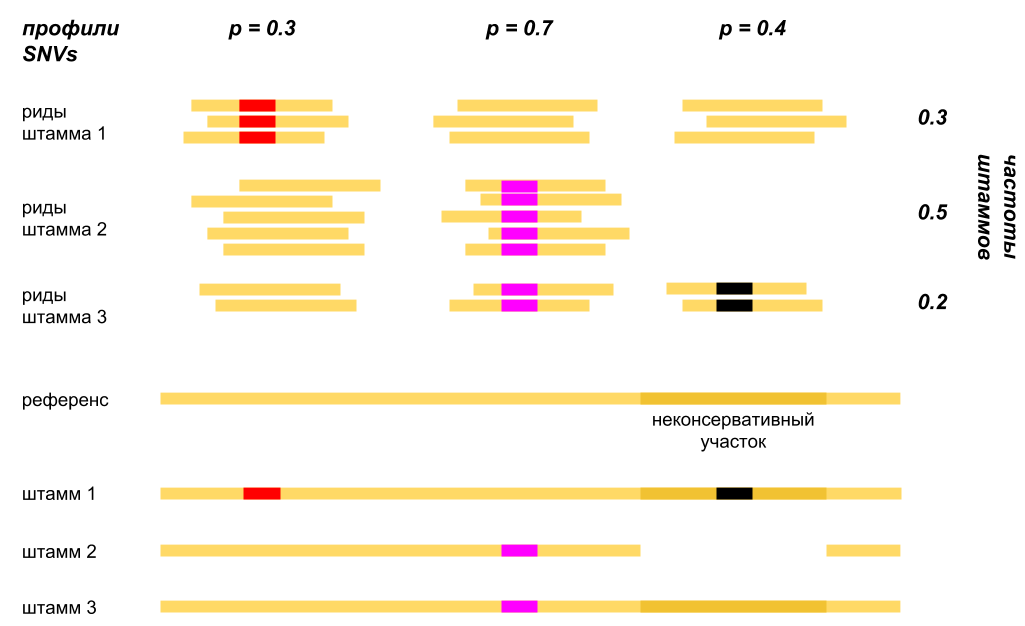
\includegraphics[width=0.9\textwidth]{pics/snv_profiles.png}
\caption{Подсчёт частот однонуклеотидныx мутаций (SNVs) для одного образца}
\label{snv_profile}
\end{figure}

 
Перед тем как использовать DESMAN для анализа штаммов определенного микроорганизма пользователь должен тем или иным способом выявить набор последовательностей (контигов или генов), соответствующих ему.
DESMAN детектирует SNV относительно однокопийных консервативных генов (которые скорее всего присутствуют в каждом из штаммов в единственном экземпляре). Затем на основании частот SNV с привлечением Байесовская модели, выводится предполагаемое количество штаммов и профили глубины их покрытия. 
На следующем этапе, для каждого из неконсервативных генов (тех, которые могут отсутствовать в одном или нескольких штаммах) DESMAN предсказывает подмножество включающих его штаммов.
Отметим, что возможность определения генетического состава индивидуальных штаммов выделяет DESMAN...TODO if needed :). 

\subsection{Цель работы}
Целью данной работы является разработка пайплайна, который будет выявлять количество близкородственных штаммов в метагеномной серии, их процентное соотношение, а также для вершин графа сборки этих штаммов будет определять, какому подмножеству штаммов они принадлежат.

\subsection{Методы}
\subsection{Графы сборки}
Данная работа посвящена выяснению состава каждого из смеси близкородственных штаммов в метагеномной серии, но с использованием помимо информации о профилях SNVs, еще и информации о структуре графа метагеномной сборки. 

\textit{Графом де Брюина}, построенном по множеству строк S, называется граф, вершины которого соответствуют всем возможным (k+1)-мерам (последовательность из k+1 символов), присутствующим в S, а направленное ребро соединяет вершину $A$ с вершиной $B$ в том и только том случае, если последние $k$ символов вершины $A$ равны первым $k$ символам вершины $B$.

\textit{Сжатым графом де Брюина} будем называть, получаемый из графа де Брюина путём итеративного объединения всех таких пар вершин (u, v) таких что из u выходит единственное ребро, и оно ведет в v, а в v входит единственное ребро, и оно идёт из u. Вершины u и v удаляются из графа, и добавляется новая вершина w, входящие рёбра которой равны входящим рёбрам u, исходящие -- исходящим рёбрам v. Последовательность символов, соответствующая w, получается путём присоединения к последовательности u всех символов v, кроме первых k.

Значительно упрощая, можно считать, что граф, с которым в дальнейшем предстоит работать (граф сборки) строится 
следующим образом:
1) По множеству ридов строится граф де Брюина 
2) По графу де Брюина строится сжатый граф де Брюина
3) Так как в ридах содержатся ошибки секвенирования, далее сжатый граф де Брюина упрощается, чтобы по возможности удалить из графа структуры, порождаемые этими ошибками. 
Последовательности, соответсвующие вершинам в графе сборки, называются юнитигами.

Если все участки генома были покрыты ридами, а в процессе упрощения графа были выкинуты только ошибочные вершины, то в графе существует путь, последовательность юнитигов которого соответствует геному. После построения графа сборки сборщики ищут такие пути или хотя бы их фрагменты, чтобы объединить юнитиги в более длинные последовательности --- контиги.

На сегодняшний момент нам известен только один инструмент, использующий структуру графа сборки для анализа смесей близкородственных штаммов, --- это MaryGold \cite{MaryGold}, но он только ищет набор мест в графе, соответствующих вариациям между штаммами. 



\section{Краткое описание подхода}

В данной работе мы будем анализировать графы сборки, полученные с помощью программы metaSPAdes \cite{MetaSpades}. Настройки этапа “упрощения” графа были модифицированы с целью сохранения связей между элементами, соответствующими различным штаммам (по-умолчанию metaSPAdes стремится в первую очередь обеспечить реконструкцию наиболее высоко-представленного штамма). 

В начале мы используем DESMAN для того, чтобы найти количество штаммов и их процентное соотношение. 

Далее мы используем модуль gene-assign программы DESMAN, чтобы определить, каким штаммам принадлежат вершины графа сборки, соответствующие длинным юнитига геномов. Введение порогового значения на минимальную длину (в текущих экспериментах 1кб) позволяет: 
исключить из рассмотрения  большинство геномных повторов 
обеспечить более точное соответствие средней глубины покрытия рассматриваемых вершин среднему значению по геному.

Затем на основании структуры графа сборки, мы попытаемся уточнить полученный результат, а также  пытаемся классифицировать остальные (короткие) вершины графа.



\section{Первоначальная классификация вершин с помощью DESMAN}

\subsection{Поиск SNVs}

Вначале нужно осуществить поиск SNVs. В случае, если известен референсный геном интересующего вида, можно использовать его. Иначе можно использовать длинные контиги, которые по результатам биннинга принадлежат одному виду.

Для выравнивания ридов мы использовали программу BWA-MEM \cite{bwa_mem}. Для поиска SNVs --- инструмент VarScan \cite{VarScan}; он позволяет не только находить позиции, в которых нуклеотиды отличаются от референса, но и фильтровывать их от ошибок секвенирования, основываясь на статистических тестах.
Отдельно отметим, что на этом этапе можно оценить, присутствует ли в принципе в образцах смесь близкородственных штаммов интересующего вида (см. Приложение  \ref{dominated_samples}).

\subsection{Фильтрация SNVs} (Пока пропустил его)

Чтобы правильно вывести из частот SNVs частоты штаммов, нужно брать только те позиции в геноме, которые не попадают на плохо покрытые участки, не принадлежат повторам и при этом присутствуют во всех штаммах рассматриваемого вида (см. пример на Рис. \ref{snv_profile}). Чтобы выполнить последние два условия, DESMAN ищет в контигах однокопийные консервативные гены и рассматривает мутации только в них. Авторы предлагают самостоятельно составлять базу таких генов для видов с большим количеством известных геномов (в своей статье они нашли 982 таких гена для E.Coli), а в случае, если доступных геномов мало, смотреть только на 36 генов, консервативных и однокопийных практически для всех прокариот. Но наши эксперименты (подробнее в \ref{infant_gut_section}) показали, что в случае, когда штаммы не слишком сильно отличаются друг от друга, в этих 36 генах случается мало мутаций, и из-за этого результаты для профилей частот штаммов оказываются неудовлетворительными. Поэтому мы ищем мутации во всём геноме и после этого фильтруем их.

Мы считаем медиану покрытия всех найденных позиций с SNVs в каждом образце, предполагая, что она отражает реальное покрытие всех штаммов рассматриваемого вида в совокупности. Таким образом нам нужны позиции с SNVs, суммарное покрытие которых близко к медиане в каждом из образцов. Мы считаем евклидово расстояние между медианой и покрытием для каждой позиции и берём 3000 самых лучших (но это число можно менять в зависимости от условий, таких как степень родства штаммов и количество образцов).

\subsection{Количество штаммов и профили их частот}

Имея вектора частот SNVs, мы можем вывести процентное соотношение с помощью одного из инструментов, упомянутых во введении. В данном случае мы используем DESMAN, как наиболее эффективный и хорошо зарекомендовавший себя (?)строгий метод из всех доступных. 

Для модели DESMAN количество штаммов в образцах является входным параметром. Но авторы предлагают использовать график среднего апостериорного отклонения для того, чтобы понять, начиная с какого количества штаммов отклонение перестаёт значительно уменьшаться. В наших экспериментах этот метод хорошо сработал как для синтетических, так и для реального датасетов (подробнее в ССЫЛКИ).

\subsection{Классификация вершин графа сборки}

В оригинальной работе авторы DESMAN полученные пропорции штаммов в образцах предлагают использовать для классификации по штаммам однокопийных неконсервативных генов на основе их покрытия, также используя Байесовский подход. Так как для использования этой процедуры необходима только информация о профилях покрытия для набора фрагментов, в данной работе мы применяем эту процедуру к длинным юнитигам. 

Так как при построении графа сборки metaSPAdes считает и сохраняет количество всех найденных k~-меров, мы можем использовать эту информацию для быстрой оценки нуклеотидного покрытия вершин по формуле $\frac{C_k r}{r - k + 1}$, где $C_k$ --- k-мерное покрытие, а $r$ -- длина ридов. Но в случае, если риды имеют большой разброс по длине, лучший результат достигается с использованием процедуры выравнивания ридов (нами используется утилита bedtools genomecov \cite{bedtools}).


\section{Валидация и типичные проблемы в результатах DESMAN}

Для разработки и валидации алгоритма нам нужны были синтетические данные, которые обычно в метагеномных исследованиях получают путём симуляции ридов из набора референсных геномов. 
Но чтобы приблизить данные к реальным экспериментам (эффекты от ошибок секвенирования, распределение покрытия), мы в данной работе симулировали данные, получая их путём смешивания в разных пропорциях коротких ридов из секвенирований разных изолятов \textit{Escherichia coli}, в рамках одного и того же геномного проекта (PRJNA239027 в базе NCBI BioProject). Авторы данной работы \cite{isolates} исследовали 6 изолятов \textit{E.coli}, присутствующие у 6 пациентов с разной степенью заражения крови. Кроме коротких ридов они провели секвенирование и сборку тех же изолятов с помощью PacBio технологии, и эти сборки мы использовали как референсные значения, к которым стремились.

Мы сгенерировали случайным образом профили частот штаммов (СДЕЛАТЬ ТАБЛИЧКИ в приложении) таким образом, чтобы каждый штамм имел существенное покрытие хотя бы в одном образце. Мы рассматривали от 2 до 5 штаммов в 10 образцах, по 2 эксперимента на каждое количество штаммов с суммарным покрытием XXX в каждом образце. Покрытие одного изолята (ИМЯ) в изначальном эксперименте оказалась низким (УКАЗАТЬ СРЕДНЕЕ), и мы не брали его риды для симуляции.

Чтобы проверять результат получившейся классификации вершин, мы прикладывали рефенс к графу таким образом, чтобы он представлял в графе связный путь везде, где это возможно; для этого мы использовали внутренние инструменты лаборатории (что здесь дописать???). Таким образом для каждой вершины графа нам было известно, в каких штаммах и с каким числом копий она встречается.

Чтобы оценить результат количественно, мы рассматривали его как ответ на задачу бинарной классификации отдельно для каждого штамма (принадлежит вершина штамму или нет).

Наши эксперименты показали, что на тестовых данных DESMAN даёт не много ложноположительных результатов на длинных вершинах. Исключения составляют вершины, соответствующие повторам, так как у них покрытие больше, чем предполагает модель. Гораздо чаще DESMAN делает ложноотрицательные выводы, и мы будем бороться в первую очередь с такими типами ошибок. Также мы будем дополнять ответ для коротких вершин.



\section{Уточнение классификации с использованием структуры графа}
\subsection{Однозначное продолжение пути в графе}
После первоначальной классификации с помощью DESMAN мы получили для каждого штамма набор длинных вершин, которые, как показало тестирование, с большой вероятностью ему принадлежат. Каждая из этих вершин должна лежать на пути в графе, образующем геном штамма. Поэтому если мы найдём, какие ещё вершины однозначно лежат на этом пути, мы сможем сказать, что с большой вероятностью они тоже принадлежат данному штамму.

Многие вершины имеют исходящую степень больше 1. Следовательно, через такую вершину существует несколько продолжений пути. В таком случае будем рассматривать один из двух вариантов. Вариант первый --- пути, выходящие из вершины, образуют \textit{пузырь}, то есть идут по разным вершинам, но потом вновь сходятся в одну (более строгое определение будет дано ниже). Тогда, если мы перескочим через этот пузырь, вершина на его конце тоже должна принадлежать рассматриваемому штамму, так как через неё однозначно проходят все возможные пути (см. Рис. \ref{bubbles_chain}). Кроме пузырей в графе существуют более сложные структуры, соответствующие повторяющимся участкам геномов, и пути через них уже не будут сходиться в одну вершину. Таким образом, если мы будем идти по графу вперёд, начиная от вершины, принадлежащей рассматриваемому штамму, то, пока нам на пути будут попадаться только пузыри, вершины между пузырями мы можем определять тоже как принадлежащие этому штамму. То же соображение работает, если мы будем идти от вершины назад по обратным рёбрам (см. Рис. \ref{bubbles_chain}).

\begin{figure}[t]
\centering
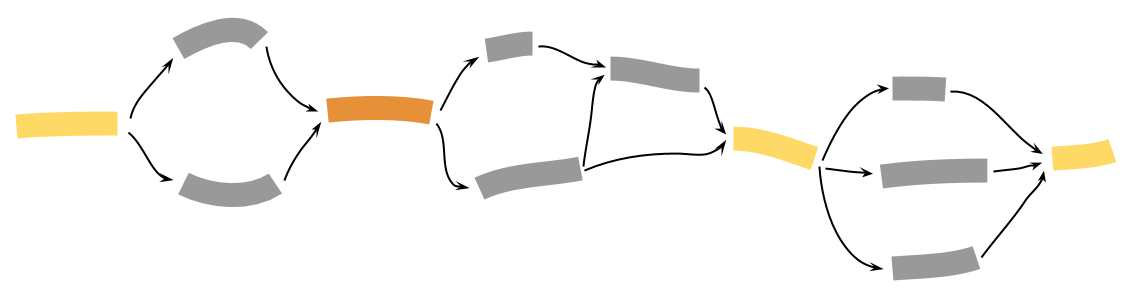
\includegraphics[width=0.8\textwidth]{pics/bubbles_chain.png}
\caption{Цепочка пузырей. Если оранжевая вершина принадлежит штамму, то жёлтые тоже должны ему принадлежать.}
\label{bubbles_chain}
\end{figure}

Чтобы искать пузыри и вершины между ними, мы воспользовались алгоритмом из статьи ССЫЛКА. Авторы данной работы вводят понятие \textit{суперпузыря} следующим образом: если упорядоченная пара вершин $(s,t)$ удовлетворяет следующим свойствам:
1) $t$ достижима из $s$;
2) набор вершин, достижимых из $s$ без прохождения через вершину $t$ равняется набору вершин, из которых достижима $t$ без прохождения через вершину $s$;
3) подграф, индуцированный набором $U$ вершин из предыдущего условия, --- ацикличен;
4) ни одна вершина из $U$, кроме $t$, не образует с $s$ пары, удовлетворяющей предыдущим условиям; то тогда множество вершин $U \cup \{s,t\}$ образуют \textit{суперпузырь}, а $s$ и $t$ --- это его начало и конец соответственно. Авторы предлагают алгоритм, основанный на стандартной топологической сортировке, который для каждой вершины за константное время в среднем определяет, является ли она началом \textit{суперпузыря} $s$, и если это так, находит его конец.

Таким образом, мы стартуем от вершины, которая принадлежит штамму, и проверяем, является ли она началом пузыря. Если это так, помечаем её конец тоже как принадлежащий штамму и итеративно продолжаем эту процедуру уже от него. То же самое мы делаем по обратным рёбрам графа.


Также мы можем проверить, нет ли среди вершин каждого штамма (в том числе тех, которые мы добавили, перескакивая пузыри) таких, что их исходящая степень равна 1. Тогда вершины, следующие за ними, тоже можно определить к этому же штамму (см Рис. \ref{one_continue}).

\begin{figure}[t]
\centering
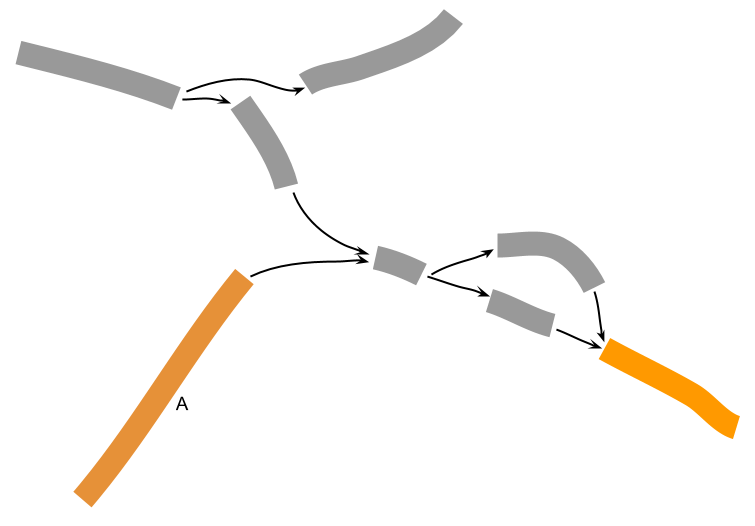
\includegraphics[width=0.57\textwidth]{pics/one_continue.png}
\caption{У вершины $A$ только одно продолжение}
\label{one_continue}
\end{figure}


\subsection{Пузыри в графе}

После того, как мы найдём цепочки пузырей и добавим к классификации их концов недостающие штаммы, мы можем сказать, какое подмножество штаммов должно проходить через каждый из пузырей. Тогда мы можем уточнить классификацию вершин внутри пузыря, основываясь на их покрытии.

Каждый штамм в пузыре соответствует пути между его началом и концом. Мы можем перебрать все варианты путей и их соответствий штаммам, чтобы найти, какой набор путей наилучшим образом объясняет наблюдаемые покрытия вершин. Разумеется, количество возможных путей растёт экспоненциально с увеличением числа вершин в пузыре, (ЗДЕСЬ НАДО ВСТАВИТЬ ГИСТОГРАММУ РАСПРЕДЕЛЕНИЯ КОЛИЧЕСТВА ВЕРШИН В РЕАЛЬНОМ И СИМУЛИРОВАННОМ ГРАФАХ И РАСПРЕДЕЛЕНИЕ КОЛИЧЕСТВА ВОЗМОЖНЫХ ПУТЕЙ).

Задача, схожая с поставленной, рассматривалась в серии работ, посвященных реконструкции альтернативных изоформ эукариотических генов на основании серий экспериментов транскриптомного секвенирования (RNA-seq) \cite{flipflop2, other_flows, flipflop1}. Как здесь нам нужно определить, какому набору штаммов принадлежит вершина, так при РНК-секвенировании нужно находить, в какие изоформы входит тот или иной экзон.


ЗДЕСЬ ЕЩЁ НАПИСАТЬ, КАК ПОНИМАТЬ, КАКОЙ НАБОР ПУТЕЙ НАИЛУЧШИМ ОБРАЗОМ ОБЪЯСНЯЕТ ПОКРЫТИЕ

\subsection{Итоговый алгоритм}

ОФОРМИТЬ ВСЁ ВЫШЕСКАЗАННОЕ В ПСЕВДОКОД



\section{Результаты}
\subsection{Простые датасеты из смесей изолятов}
\subsection{Датасет Strain Mock}
\subsection{Реальный датасет} \label{infant_gut_section}

ТЕЗИСЫ:

В данном исследовании авторы нашли в рассматриваемых образцах три штамма S.epidermidis. Авторы посчитали процентное соотношение этих штаммов и сделали качественные сборки двух из них (НАПИСАТЬ, КАКИМ ОБРАЗОМ).

В предыдущей работе, до того, как была опубликована статья про DESMAN, мы уже анализировали частоты SNVs, чтобы определить процентное соотношение штаммов. Мы кластеризовали профили частот и смотрели на центры кластеров --- можно ли центры одних кластеров представить как сумму других, соответствующих мутациям только одного штамма. Наш анализ выявил, что в данных присутствует четыре штамма, а профили частот в некоторых образцах отличаются от заявленных в исследовании. Анализ с помощью DESMAN подтвердил наши результаты (НАПИСАТЬ ЕЩЕ, ЧТО 36 ГЕНОВ НЕ ОК). Кроме того мы нашли в графе сборке две длинные вершины (УКАЗАТЬ ДЛИНУ), которые не выравниваются на strain1 и strain3, но судя по выравниванию на базу NCBI точно принадлежат S.epidermidis, и их покрытие также соотносится с нашими результатами.

Из графа сборки этих данных не получается однозначно выделить компоненту, принадлежащую S.epidermidis, так как в образцах присутствует родственный ему вид ???. Поэтому, чтобы уменьшить потенциальное количество вершин, мы сделали следующее: мы провели биннинг длинных вершин (больше 1000 баз) с помощью CONCOCT. Дальше мы выравняли сборки из статьи на граф и выкинули те длинные вершины, которые не выравнивались на S.epidermidis и принадлежали бинам, в которых его было меньше 30\%. После этого мы оставили только компоненту слабой связности, которой принадлежали все вершины S.epidermidis. В получившемся графе мы удалили все короткие тупики (меньше 500 баз) и сжали вместе все вершины, которые можно было соединить. Таким образом мы сузили количество рассматриваемых вершин и упростили граф, но, скорее всего, не потеряли вершины, которые принадлежат S.epidermidis. Выравнивание длинных вершин на базу NCBI показало, что мы включили в анализ как вершины, принадлежищие S.epidermidis (но которых нет в сборках статьи), так и вершины плазмид и фагов S.epidermidis, плюс небольшое количество вершин родственного вида. Но нашей целью является поиск штаммо-специфичных вариаций, которые могли бы в дальнейшем объяснить фенотипические различия, поэтому мы исходим из того, что лучше добавить в анализ лишние вершины, чем потерять нужные.




% У заключения нет номера главы
\section*{Заключение}
В данной работе






\bibliographystyle{ugost2008ls}
\bibliography{diploma.bib}

%\appendix
\begin{appendices}

\section{Поиск смесей штаммов в образцах}\label{dominated_samples}

ПЕРЕПИСАТЬ

Опишем алгоритм поиска образцов с доминантными штаммами некоторого рассматриваемого вида.

В каждом образце найдем однонуклеотидные мутации относительно референса рассматриваемого вида. Для каждой мутации считаем, сколько ридов поддерживает референс, а сколько – мутацию. Чтобы оставить только те мутации, которые не лежат в повторах и малопокрытых участках генома, возьмем только такие, чье суммарное покрытие близко к медиане покрытия этого вида в образце. Для каждой из выбранных мутаций подсчитаем частоту ридов, поддерживающих мутацию.

Каждая мутация специфична для какого-то одного штамма или некоторого множества штаммов. Если мы выбрали мутации с хорошим покрытием и не попадающие в повторы, то частота ридов, поддерживающих эту мутацию, должна примерно соответствовать сумме частот штаммов, для которых специфична эта мутация.

Тогда заметим, что если частота доминантного штамма – X, и X > 0.7, то мы должны наблюдать мутации с частотой порядка X и больше. При этом мутации, специфичные только для всех остальных штаммов, не могут давать частоты больше (1-X). Тогда в случае, когда в образце присутствует доминантный штамм, в распределении частот, соответствующих мутациям, мы должны наблюдать отсутствие значений в промежутке ((1-X); X).

Найдем величину промежутка эмпирически. Так как границы промежутка должны быть симметричны относительно значения 0.5, начнем с его середины и будем добавлять с обоих концов некоторую маленькую величину eps (например, 0.01) до тех пор, пока в промежуток попадает не больше 5\% от всех значений частот мутаций (те мутации, которые туда попали, считаем погрешностью). После того, как мы нашли предполагаемый промежуток, смотрим на его правую границу. Если она больше 0.7, считаем, что X > 0.7, и в образце есть доминантный штамм. Иначе – доминантного штамма нет.


\section{приложение два}
текст

\end{appendices}

\end{document}
